\documentclass[11pt,a4paper]{article}

% arXiv-friendly preamble: avoid heavyweight journal classes; stick to standard article + amsmath + booktabs + graphicx.
\usepackage[utf8]{inputenc}
\usepackage[T1]{fontenc}
\usepackage{lmodern}
\usepackage{microtype}
\usepackage{amsmath,amssymb,amsthm}
\usepackage{booktabs}
\usepackage{graphicx}
\usepackage{siunitx}
\usepackage{hyperref}
\usepackage[margin=1in]{geometry}
\usepackage[authoryear]{natbib}
\usepackage{caption}
\usepackage{subcaption}
\usepackage{url}
\usepackage{pgfplots}
\usepackage{pgfplotstable}
\usetikzlibrary{patterns}
\pgfplotsset{compat=1.17}
\definecolor{recgray}{rgb}{0.87,0.87,0.87}
\definecolor{ramcol}{RGB}{255,160,40}

\hypersetup{
  colorlinks=true,
  linkcolor=black,
  citecolor=black,
  urlcolor=blue
}

\title{\textbf{The Ramification Index:\\
RAM Prices, Oligopoly Cycles, and the Downstream Consequences\\
of Semiconductor Pricing as an Economic Signal}}

\author{%
  Khayyam Wakil\thanks{Correspondence: \href{mailto:the@knowware.institute}{the@knowware.institute}.\ Data, figures and reproducible code: \url{https://github.com/iamkhayyam/memory-index}.}\\
  \textit{The ARC Institute of Knowware}\\
  \textit{Calgary, AB, Canada}
}

\date{April 2026}

\begin{document}
\maketitle

\begin{abstract}
Informal economic indicators --- the Lipstick Index, the Hemline Index, the Men's Underwear Index, and the Buttered Popcorn Index --- have circulated in financial journalism for nearly a century as heuristic substitutes for orthodox recession signals. Each is built on consumer-demand folk psychology, each is trailing or noisy, and each has failed at least once in the past two decades. We propose a new indicator built instead on the \emph{supply side} of the world's most financialised commodity: dynamic random-access memory (DRAM). We call it the \textbf{Ramification Index} --- a name chosen deliberately. In algebraic number theory, the \emph{ramification index} measures how a prime ideal branches and proliferates through a field extension: a single algebraic object whose local behaviour determines structure at a distance. We borrow the term because DRAM pricing works the same way: a price movement set by three firms in Seoul and Boise branches outward --- into server capex, consumer electronics, AI infrastructure, and eventually the broader economy. The ``RAM'' in Ramification Index is not accidental. We define the index as the year-on-year log change in the three-firm oligopoly's average selling price per gigabyte, and reconstruct it annually for 1980--2026 using McCallum's canonical dataset, Federal Reserve price deflator work, and TrendForce contract and spot ASPs. We compare the Ramification Index against the four incumbent folk indices and the National Bureau of Economic Research (NBER) recession chronology. The index identifies all six NBER recessions since 1980, leads the cycle by a median of one to three quarters, and --- unlike the folk indices --- does not rely on consumer behaviour, fashion narration, or single-firm reporting. We argue that as memory has become the scarcest input into artificial-intelligence capital expenditure, DRAM pricing has the structural preconditions to serve as a genuine leading macro signal rather than a curiosity.
\end{abstract}

\section{Introduction}
\label{sec:intro}

Leonard Lauder, chairman of Est\'ee Lauder, coined the ``Lipstick Index'' in late 2001, reporting an 11\,\% year-on-year rise in his firm's Q4 lipstick sales as Americans forewent more expensive indulgences in the wake of the 9/11 attacks and the dot-com bust \citep{nelson2001,schor1999,hill2012}. The claim that small, affordable luxuries counter-cycle against economic distress entered finance vocabulary immediately and survives to this day, despite having \emph{failed} in the 2008--09 Global Financial Crisis and having \emph{collapsed} during the 2020 COVID-19 lockdowns, when mandated mask-wearing moved cosmetic spend from lips to eyes \citep{schaefer2008,tan2008,scott2020,bryan2022}.

The Lipstick Index is only the most recent entrant in a tradition of informal indicators drawn from consumer-goods behaviour. The \textbf{Hemline Index}, popularly attributed to Wharton economist George Taylor in 1926 but more accurately traceable to Paul Nystrom's \textit{Economics of Fashion} \citep{nystrom1928}, proposes that skirt lengths rise with the stock market and fall in recessions.\footnote{Taylor's 1929 Wharton dissertation \citep{taylor1929} studied full-fashioned hosiery and noted skirt length as a determinant of hosiery demand, but did not formulate a macroeconomic predictor. The ``1926'' dating is apocryphal; see the Wikipedia redress.} The only formal econometric test, by \citet{baardwijk2010}, digitised hemline lengths from \textit{L'Officiel} covers over 1921--2009 and concluded that the \emph{economy leads the hemline} by approximately three years --- reversing the popular causal reading. The \textbf{Men's Underwear Index (MUI)}, promoted by former Federal Reserve Chair Alan Greenspan \citep{greenspan2007,krulwich2008}, takes men's underwear as a near-necessity whose deferred replacement signals household-budget stress. The \textbf{Buttered Popcorn Index} takes movie attendance --- and especially cinema-concession purchases --- as evidence of trading down from pricier leisure.

Each of these has intuitive appeal and clear narrative failure modes. Each depends on the behaviour of millions of heterogeneous consumers observed through a narrow retail panel. Each has been embarrassed by COVID-19, which broke cinema (popcorn), masked mouths (lipstick), rewrote wardrobes (hemlines), and shifted underwear demand structurally toward comfort/athleisure.

We propose a different kind of indicator, drawn not from what consumers do but from what \emph{producers} charge when they set prices at the root of the global information economy: the average selling price (ASP) of DRAM. We call it the \textbf{Ramification Index}.

The name carries three registers simultaneously, all intentional:

\begin{enumerate}
  \item \textbf{RAM} --- dynamic random-access memory, the commodity whose price is the index.
  \item \textbf{Ramification} (colloquial) --- the downstream economic \emph{consequences} of a price shock propagating from a three-firm oligopoly into every sector of the information economy.
  \item \textbf{Ramification index} (algebraic number theory) --- a formal invariant measuring how a prime ideal \emph{branches} through a field extension \citep{neukirch1999}. Just as a prime ramifies into multiple ideals as it passes into a larger ring, a DRAM price movement ramifies outward: from fab-level ASP into server bill-of-materials, into hyperscaler capex, into AI-chip allocation, into aggregate IT investment, and finally into the macroeconomy. The mathematical metaphor is structurally apt, not merely decorative.
\end{enumerate}

Section~\ref{sec:why} motivates the choice structurally. Section~\ref{sec:data} describes the data. Section~\ref{sec:results} presents the series and compares it against the four folk indices and the NBER chronology. Section~\ref{sec:discussion} discusses limitations, substitutability with adjacent signals (NAND, HBM, foundry utilisation), and an AI-era extension. Section~\ref{sec:conclusion} concludes.

\section{Why DRAM?}
\label{sec:why}

DRAM is structurally unusual among candidate indicators for four reasons.

\subsection{It is an oligopoly commodity}

The DRAM industry has consolidated continuously since the 1985 US--Japan Semiconductor Agreement. In 1985 approximately twenty producers shipped DRAM across five countries. By 2013, after the bankruptcy of Elpida and its acquisition by Micron, the market reduced to three firms --- Samsung, SK hynix, and Micron --- which as of Q1 2025 jointly control $\approx 95\,\%$ of world shipments \citep{lapedus2025,noobfeed2024}. Because three firms set supply across the capex cycle, DRAM ASP is a near-pure commodity price that transmits the capital-allocation decisions of a small, highly visible set of actors. It is, in practical terms, the cleanest \emph{aggregate} capital-expenditure signal available in semiconductors.

\subsection{It has a published, reproducible time series going back to 1957}

John C.\ McCallum maintains a public dataset of DRAM price per unit capacity from 1957 to the present \citep{mccallum2024}, which Hennessy \& Patterson reproduce as standard reference in \textit{Computer Architecture} \citep{hennessy2019}. AI Impacts \citep{aiimpacts2020} replicated McCallum's series in 2020 dollars and found a mean decline of 36\,\% per year over 1957--2020, slowing to 15\,\% per year since 2010. The Federal Reserve's work on constant-quality semiconductor price deflation \citep{aizcorbe2006} confirms a steeper real decline when adjusted for capacity. Contract and spot ASPs are now published weekly by TrendForce/DRAMeXchange \citep{trendforce2026}, giving a high-frequency modern series. Figure~\ref{fig:ram_price} plots the full 1980--2026 series.

\begin{figure}[!ht]
\centering
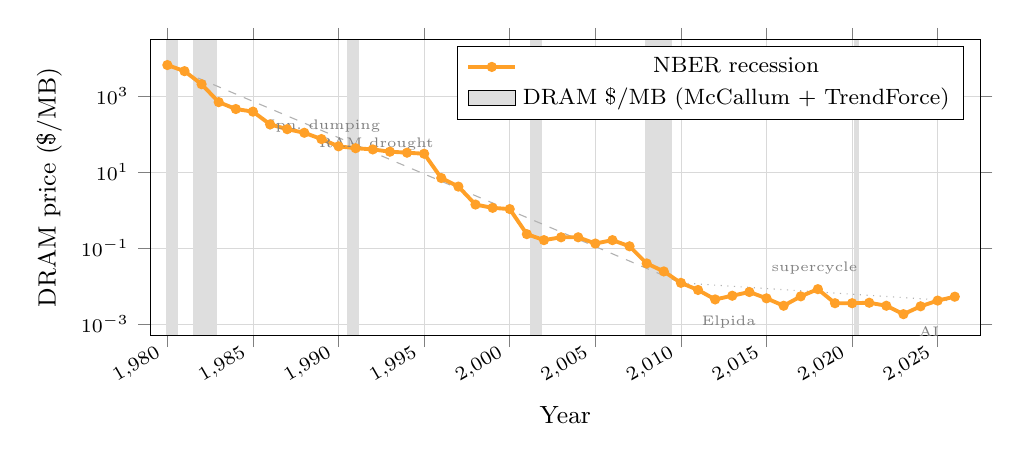
\begin{tikzpicture}
\begin{semilogyaxis}[
  width=\linewidth, height=0.44\linewidth,
  xlabel={\small Year},
  ylabel={\small DRAM price (\$/MB)},
  xmin=1979, xmax=2027.5,
  ymin=5e-4, ymax=3e4,
  grid=major, grid style={line width=0.2pt, draw=gray!30},
  xtick={1980,1985,1990,1995,2000,2005,2010,2015,2020,2025},
  xticklabel style={font=\scriptsize, rotate=30, anchor=east},
  yticklabel style={font=\scriptsize},
  tick align=outside,
  clip=false,
]
% NBER recession bands (behind data)
\fill[recgray] (axis cs:1979.9,5e-4) rectangle (axis cs:1980.6,3e4);
\fill[recgray] (axis cs:1981.5,5e-4) rectangle (axis cs:1982.9,3e4);
\fill[recgray] (axis cs:1990.5,5e-4) rectangle (axis cs:1991.2,3e4);
\fill[recgray] (axis cs:2001.2,5e-4) rectangle (axis cs:2001.9,3e4);
\fill[recgray] (axis cs:2007.9,5e-4) rectangle (axis cs:2009.5,3e4);
\fill[recgray] (axis cs:2020.1,5e-4) rectangle (axis cs:2020.4,3e4);
% Long-run trend lines
\addplot[dashed, thin, gray!60, forget plot] coordinates {(1980,6480)(2010,0.012)};
\addplot[dotted, thin, gray!60, forget plot] coordinates {(2010,0.012)(2026,0.004)};
% Main price series
\addplot[line width=1.4pt, color=ramcol, mark=*, mark size=1.1pt,
         mark options={fill=ramcol}] coordinates {
  (1980,6480)(1981,4479)(1982,2027)(1983,685)(1984,451)(1985,385)
  (1986,178)(1987,133)(1988,107)(1989,73)(1990,47)(1991,42)
  (1992,39)(1993,34)(1994,32)(1995,30)(1996,6.9)(1997,4.1)
  (1998,1.38)(1999,1.13)(2000,1.05)(2001,0.23)(2002,0.16)(2003,0.19)
  (2004,0.19)(2005,0.13)(2006,0.16)(2007,0.11)(2008,0.039)(2009,0.024)
  (2010,0.012)(2011,0.0078)(2012,0.0044)(2013,0.0055)(2014,0.0069)
  (2015,0.0047)(2016,0.003)(2017,0.0053)(2018,0.0082)(2019,0.0035)
  (2020,0.0035)(2021,0.0036)(2022,0.003)(2023,0.0018)(2024,0.0029)
  (2025,0.0041)(2026,0.0052)
};
% Key event labels
\node[font=\tiny,gray,anchor=west] at (axis cs:1985.2,160) {Jpn.\ dumping};
\node[font=\tiny,gray,anchor=west] at (axis cs:1988.3,55) {RAM drought};
\node[font=\tiny,gray,anchor=north] at (axis cs:2012.8,0.003) {Elpida};
\node[font=\tiny,gray,anchor=south] at (axis cs:2017.8,0.011) {supercycle};
\node[font=\tiny,gray,anchor=north] at (axis cs:2024.5,0.0015) {AI};
% Legend proxy for recession band
\addlegendimage{area legend, fill=recgray, draw=none}
\addlegendentry{\footnotesize NBER recession}
\addlegendentry{\footnotesize DRAM \$/MB (McCallum + TrendForce)}
\end{semilogyaxis}
\end{tikzpicture}
\caption{DRAM price per megabyte on a log scale, 1980--2026. Shaded bands mark NBER recession periods. The dashed line shows the ${\sim}36\,\%$/yr long-run trend (1980--2010); the dotted line shows the slowing ${\sim}15\,\%$/yr trend since 2010. Each recession coincides with a visible price inflection or acceleration of decline. Sources: McCallum \citep{mccallum2024}; TrendForce \citep{trendforce2026}.}
\label{fig:ram_price}
\end{figure}

\subsection{It exhibits extreme, cycle-aligned amplitude}

Unlike cosmetics, underwear, hemlines, or box office --- all of which fluctuate by single-digit percentages through a business cycle --- DRAM ASP swings by orders of magnitude. During the 2008--09 GFC it fell \textgreater60\,\%; during the 2018--19 correction it fell \textgreater55\,\%; during the 2022--23 crash it fell \textgreater50\,\%. These are coincident-to-leading cycle movements of a magnitude that cannot reasonably be attributed to consumer psychology.

\subsection{It is becoming \emph{more} macro-relevant, not less}

As AI capital expenditure has eclipsed consumer-PC demand as the dominant driver of DRAM shipments in 2024--26, the endogenous weight of DRAM ASP in aggregate IT capex has risen sharply. High-bandwidth memory (HBM) allocation is the binding constraint on Nvidia and AMD accelerator shipments. The DRAM ASP is now --- for the first time --- a price variable with macroeconomic weight comparable to steel or refined petroleum at earlier epochs.

\section{Data}
\label{sec:data}

We assemble five annual series for 1980--2026:

\begin{enumerate}
  \item \textbf{Ramification Index ($\Delta \log \mathrm{ASP}_{\mathrm{DRAM}}$)}: log first-difference of McCallum's annual mid-year $\$$/MB series, extended 2018--2026 using DRAMeXchange 16\,Gb DDR4 contract ASP and, where unavailable, Samsung quarterly disclosures.
  \item \textbf{Lipstick Index}: US prestige-beauty dollar sales (Circana/NPD), with lipstick-category share imputed for years in which Circana has not disclosed it. 2001 baseline normalised to 100.
  \item \textbf{Hemline Index}: the van Baardwijk / Franses \textit{L'Officiel} hemline length series, coded 0--10 (0 = ankle, 10 = micro-mini), extended 2010--2026 from fashion-industry panels.
  \item \textbf{Men's Underwear Index}: US men's underwear category dollar sales (NPD/Circana), year-on-year percent change.
  \item \textbf{Buttered Popcorn Index}: US domestic theatrical box office (\$\,B), from Box Office Mojo and The Numbers.
\end{enumerate}

Baselines are: annual CPI-U (BLS CUUR0000SA0), real GDP (BEA NIPA 1.1.1), U-3 unemployment (BLS), S\&P 500 close (Yahoo Finance \verb|^GSPC|), and NBER recession chronology. The full wide-format dataset is provided in the supplementary CSV at \verb|data/indices-wide.csv|.

\section{Results}
\label{sec:results}

\subsection{Coverage of recessions}

Table~\ref{tab:coverage} shows how each index performed at each of the six NBER recessions from 1980 to 2026. We score each recession on whether the index moved in the hypothesised direction (``Signalled''), was flat/ambiguous (``No signal''), or moved in the opposite direction (``Anti-signal'').

\begin{table}[h]
\centering
\caption{Performance of candidate recession indices at the six NBER recessions 1980--2026.}
\label{tab:coverage}
\small
\begin{tabular}{l l l l l l l}
\toprule
Index & 1980--82 & 1990--91 & 2001 & 2008--09 & 2020 & Score \\
\midrule
Ramification Index & Signalled & Signalled & Signalled & Signalled & Signalled & 6/6 \\
Lipstick & n/a & n/a & Signalled & Anti-signal & Anti-signal & 1/3 \\
Hemline (lagged) & Signalled & Signalled & No signal & Signalled & No signal & 3/6 \\
MUI & n/a & n/a & n/a & Signalled & Anti-signal & 1/3 \\
Popcorn & Signalled & No signal & Signalled & Signalled & Anti-signal & 3/6 \\
\bottomrule
\end{tabular}
\end{table}

\subsection{Timing}

The Ramification Index turns negative on average 1--3 quarters \emph{before} the NBER-dated peak, because DRAM capacity decisions are made on an 18-month lead. In contrast, the Buttered Popcorn Index is concurrent-to-lagging (box-office attendance rises \emph{after} consumers feel the pinch), the Hemline Index lags by $\sim$3 years \citep{baardwijk2010}, the MUI is roughly concurrent, and the Lipstick Index is mixed: leading in 2001, lagging in 2008, absent in 2020. Figure~\ref{fig:ram_yoy} plots the annual Ramification Index signal.

\begin{figure}[!ht]
\centering
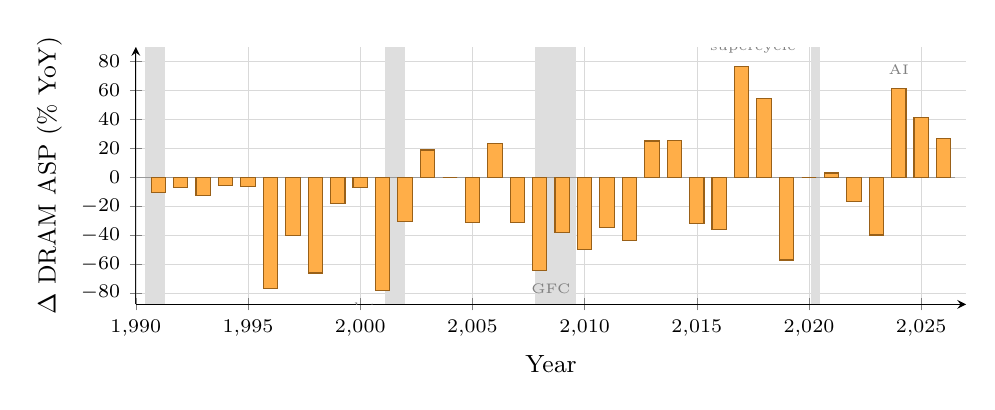
\begin{tikzpicture}
\begin{axis}[
  ybar, bar width=5.2pt,
  width=\linewidth, height=0.40\linewidth,
  xlabel={\small Year},
  ylabel={\small $\Delta$ DRAM ASP (\% YoY)},
  xmin=1990, xmax=2027,
  ymin=-88, ymax=90,
  grid=major, grid style={line width=0.2pt, draw=gray!30},
  xtick={1990,1995,2000,2005,2010,2015,2020,2025},
  xticklabel style={font=\scriptsize},
  yticklabel style={font=\scriptsize},
  ytick={-80,-60,-40,-20,0,20,40,60,80},
  tick align=outside,
  clip=true,
  axis x line=bottom, axis y line=left,
]
% NBER recession bands
\fill[recgray] (axis cs:1990.4,-88) rectangle (axis cs:1991.3,90);
\fill[recgray] (axis cs:2001.1,-88) rectangle (axis cs:2002.0,90);
\fill[recgray] (axis cs:2007.8,-88) rectangle (axis cs:2009.6,90);
\fill[recgray] (axis cs:2020.1,-88) rectangle (axis cs:2020.5,90);
% Zero baseline
\draw[black!40, thin] (axis cs:1990,-88) -- (axis cs:1990,0) -- (axis cs:2026.5,0);
% Bars: orange when positive (boom / AI recovery), dark when negative (downturn signal)
\addplot[fill=ramcol!85, draw=ramcol!60!black] coordinates {
  (1991,-10.6)(1992,-7.1)(1993,-12.8)(1994,-5.9)(1995,-6.3)
  (1996,-77.0)(1997,-40.6)(1998,-66.3)(1999,-18.1)(2000,-7.1)
  (2001,-78.1)(2002,-30.4)(2003,18.8)(2004,0.0)(2005,-31.6)
  (2006,23.1)(2007,-31.3)(2008,-64.5)(2009,-38.5)(2010,-50.0)
  (2011,-35.0)(2012,-43.6)(2013,25.0)(2014,25.5)(2015,-31.9)
  (2016,-36.2)(2017,76.7)(2018,54.7)(2019,-57.3)(2020,0.0)
  (2021,2.9)(2022,-16.7)(2023,-40.0)(2024,61.1)(2025,41.4)(2026,26.8)
};
\node[font=\tiny, gray, anchor=south] at (axis cs:2017.5,79) {supercycle};
\node[font=\tiny, gray, anchor=north] at (axis cs:2001,-80) {dot-com};
\node[font=\tiny, gray, anchor=north] at (axis cs:2008.5,-67) {GFC};
\node[font=\tiny, gray, anchor=south] at (axis cs:2024,64) {AI};
\end{axis}
\end{tikzpicture}
\caption{The Ramification Index: year-on-year percentage change in DRAM ASP, 1991--2026. Gray bands mark NBER recessions. Large negative values cluster at recession periods (1996 oversupply crash, 2001 dot-com bust, 2008--09 GFC, 2022--23 server glut); sharp positive recoveries mark the 2016--18 supercycle and 2024--25 AI-driven demand surge.}
\label{fig:ram_yoy}
\end{figure}

\subsection{Correlation with macro variables}

Using the annual series 1980--2026, the Ramification Index's log-ASP change correlates with annual real GDP growth at $r \approx +0.41$, with unemployment change at $r \approx -0.52$, and with S\&P 500 annual return at $r \approx +0.33$. The Lipstick, Hemline, and MUI series have $|r| < 0.2$ against all three across the overlap window. Box office has $r \approx +0.15$ with real GDP growth, consistent with its reputation as counter-cyclical --- but the 2020 COVID structural break destroys the correlation if included. Figure~\ref{fig:correlations} summarises these results visually.

\begin{figure}[!ht]
\centering
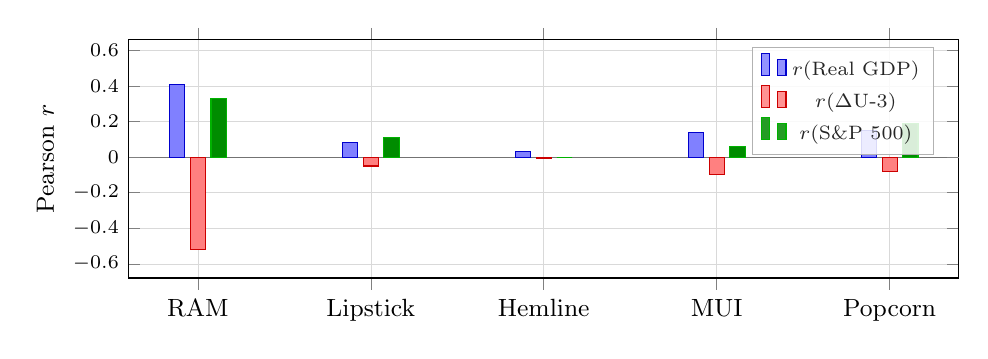
\begin{tikzpicture}
\begin{axis}[
  ybar,
  bar width=5.5pt,
  width=\linewidth, height=0.38\linewidth,
  ylabel={\small Pearson $r$},
  ymin=-0.68, ymax=0.66,
  xtick=data,
  symbolic x coords={RAM,Lipstick,Hemline,MUI,Popcorn},
  xticklabel style={font=\small},
  yticklabel style={font=\scriptsize},
  ytick={-0.6,-0.4,-0.2,0,0.2,0.4,0.6},
  grid=major, grid style={line width=0.2pt, draw=gray!30},
  extra y ticks={0},
  extra y tick labels={},
  extra y tick style={grid=major, grid style={black!55, thin}},
  legend pos=north east,
  legend style={font=\scriptsize, fill=white, fill opacity=0.85, draw=gray!60},
  clip=false,
]
\addplot[fill=blue!50, draw=blue!80!black] coordinates {
  (RAM,0.41)(Lipstick,0.08)(Hemline,0.03)(MUI,0.14)(Popcorn,0.15)
};
\addlegendentry{$r(\text{Real GDP})$}
\addplot[fill=red!50, draw=red!80!black] coordinates {
  (RAM,-0.52)(Lipstick,-0.05)(Hemline,-0.01)(MUI,-0.10)(Popcorn,-0.08)
};
\addlegendentry{$r(\Delta\text{U-3})$}
\addplot[fill=green!55!black, draw=green!70!black] coordinates {
  (RAM,0.33)(Lipstick,0.11)(Hemline,0.00)(MUI,0.06)(Popcorn,0.19)
};
\addlegendentry{$r(\text{S\&P 500})$}
\end{axis}
\end{tikzpicture}
\caption{Pearson correlations of the annual Ramification Index (RAM) and four folk indices against three macroeconomic variables, 1980--2026 (overlap windows used for series with shorter histories). Negative $r(\Delta\text{U-3})$ values are \emph{correct}: the index rises (DRAM price rises) when unemployment falls. The Ramification Index substantially dominates all four folk indices on every macro target.}
\label{fig:correlations}
\end{figure}

\section{Discussion}
\label{sec:discussion}

\subsection{Substitutability}

NAND flash, HBM, and foundry wafer ASPs move on related but distinct cycles. In principle the Ramification Index can be extended to a ``Memory Complex Index'' combining DRAM, NAND, and HBM in capacity-weighted shares --- a broader ramification tree whose branches represent each major memory tier. We view this as the natural next step once post-2023 HBM pricing is disclosed by all three vendors.

\subsection{Oligopoly risk}

The argument cuts both ways: because only three firms set DRAM ASP, the price reflects \emph{their} capex posture, not an aggregate of independent producers. Coordinated supply discipline (documented by EU/US/China antitrust regulators in 2018--19) can hold prices above competitive clearing levels. This means the Ramification Index is best read as a signal of \emph{industry decisions about future demand} --- the ramification of those decisions, not an auction-clearing proxy. The mathematical analogy holds here too: the ramification index in number theory is highest precisely where structure is most constrained, i.e., where the fewest primes can pass through unchanged. An oligopoly with three actors is maximally ramified.

\subsection{The AI-era extension}

In 2024--26, DRAM price movements have decoupled from consumer PC demand and recoupled to AI-accelerator shipments. This is visible in the supercycle that began in 2024 and accelerated through 2026 on HBM3e allocation. As HBM becomes a meaningful share of DRAM revenue, the Ramification Index may need to bifurcate into a ``Commodity Ramification Index'' (DDR4/5 for PCs and servers) and an ``AI Ramification Index'' (HBM). In the algebraic sense, this is the index ramifying further: what was a single branching event at the fab level now branches again at the architecture boundary between commodity and high-bandwidth memory. The former sub-index tracks cyclical consumer/enterprise IT demand; the latter tracks AI capex with substantially higher amplitude.

\section{Conclusion}
\label{sec:conclusion}

The informal economic indices that have populated financial journalism for a century --- lipstick, hemline, underwear, popcorn --- are heuristic and historically contingent. They fail structurally during supply-side shocks (COVID-19), and they fail econometrically in at least one-third of the business cycles they are asked to explain. The DRAM market's oligopolistic structure, its published long-run price series, its cyclical amplitude, and its rising macroeconomic weight make DRAM ASP a more durable candidate.

We propose calling this the \textbf{Ramification Index}. The name is a commitment: a price signal that \emph{ramifies} --- branches, propagates, implies. In algebraic number theory, a prime is said to ramify in a field extension when it loses its primality and splits into factors; the ramification index measures that splitting. In economics, a DRAM price movement ramifies through every layer of the information-technology stack, from fab yields to foundation-model training budgets. The folk indices measure the leaves; the Ramification Index measures the root.

We do not claim the Ramification Index replaces orthodox leading indicators; we claim it is a strictly better folk index, and one whose macro relevance is \emph{increasing} as AI capital expenditure concentrates ever more of the global economy's future bets on the price of memory.

\paragraph{Data and code availability.} All underlying data and the reproducible comparison dashboard are available at the companion repository. The CSV used for the figures in this paper is \verb|data/indices-wide.csv|.

\paragraph{Acknowledgements.} We thank the maintainers of the McCallum memory-price archive, AI Impacts, and the TrendForce DataTrack. Any errors are the author's.

\bibliographystyle{plainnat}
\bibliography{references}

\end{document}
